\documentclass[a4paper,titlepage]{report}
\usepackage[T1]{fontenc} % codifica dei font
\usepackage[utf8]{inputenc} % lettere accentate da tastiera
\usepackage[italian]{babel} % lingua del documento
\usepackage{url} % per scrivere gli indirizzi Internet
\usepackage[sans,nouppercase]{frontespizio}
\usepackage{booktabs}


\begin{document}

\begin{frontespizio}
\Universita{Verona}
\Facolta{Informatica}
\Corso[Laurea]{Informatica}
\Titoletto{Tesi di laurea}
\Titolo{Internet of Things: un progetto di smart parking}
\Candidato{Aurora Bussola}
\Relatore{Prof. Nicola Fausto Spoto}
\Annoaccademico{2021-2022}
\Rientro{1.5cm}
\NCandidato{Laureando}
\Punteggiatura{}
\end{frontespizio}

\begin{abstract}
L'evoluzione digitale ha permesso ad Internet di espandersi coinvolgendo non solo computer networks ma pure diverse tipologie di dispositivi creando un legame fra il mondo virtuale e concreto. L'innovazione coinvolge un'infinità di ambiti, per questo motivo possiamo trovare dispositivi smart fra i più disparati: dalle macchinette del caffè connesse al WiFi di casa a dispositivi biomedicali come i pacemaker\cite{Ansari:BasedHealthcareApplications}. Tutto ciò trova ragione di esistere se si va ad analizzare la natura dell'uomo e del suo ambiente: siamo circondati da cose e più in particolare sopravviviamo grazie a delle cose ed è questo motivo per cui quest'ultime dovrebbero essere più importanti di qualsiasi idea e/o informazione\cite{Ashton: ThatInternetofThings'Thing}.\\La tesi, dopo una breve parte introduttiva, prenderà in esame un parcheggio intelligente per automobili trovando una possibile soluzione con l'ausilio di una piattaforma hardware per la prototipazione che sarà costantemente connessa ad Internet. Verranno descritti in particolare tutti gli aspetti e le scelte progettuali anche attraverso schemi concettuali, immagini e pseudocodici.
\end{abstract}

\tableofcontents

\chapter{Internet of Things}
\section{Definizione}
L'{\itshape Internet of Things}  abbrev. {\itshape IoT} (oppure {\itshape Internet delle Cose}, in italiano) può essere visto come un'estensione dell'Internet da noi conosciuto che aggiunge diverse tipologie di network e sensori. Esso incrementa l'ubiquità di Internet permettendo l'interconnessione di svariate tipologie di oggetti opportunamente configurati\cite{Feng:InternationJournalOfCommunicationSystems}.
\section{Una breve storia}
Il termine {\itshape Internet of Things} è stato coniato nel 1999 da Kevin Ashton, direttore dell'Auto-ID Centre\footnote{un'organizzazione no profit con sede presso il MIT} all'interno del quale venne inventata la tecnologia {\itshape RFID} (acronimo di {\itshape Radio-Frequency IDentification}). L'invenzione soppianta il vecchio sistema barcode semplificando la gestione di beni in svariati ambiti: nel 2000 LG pianifica lo sviluppo un frigorifero intelligente in grado di {\itshape capire} se un determinato prodotto fosse presente o meno; tre anni dopo la tecnologia RFID entra nel programma SAVI\footnote{acronimo di {\itshape Navy sexual Assault Victim Interventition}, per la difesa alle vittime di tale delitto} e all'interno della grande catena di supermercati Walmart; nel 2008 viene esteso l'uso del protocollo IP a network di oggetti e nel 2011 nasce la {\itshape IPSO Alliance}, un forum di portata globale che arruola diversi colossi industriali per lo sviluppo dell’{\itshape Internet of Things}\cite{Suresh:StateArtReviewIoTHistoryTechnologyFieldsDeployment}.

\chapter{La tecnologia RFID}
\section{Definizione e funzionamento}
La tecnologia RFID, citata in precedenza, permette la lettura e/o scrittura di informazioni rigurdanti svariate tipologie di oggetti. Grazie al suo costo relativamente ridotto e al suo enorme potenziale, la tecnologia RFID viene tutt'ora largamente adoperata in progetti IoT.\\Ogni sistema RFID è composto da tre elementi: il primo è un'etichetta elettronica (tag) che memorizza l'informazione, il secondo è un apparato che si interfaccia col tag (interrogatore\footnote{solitamente è uno scrittore o un lettore}) e il terzo è un dispositivo che gestisce il collegamento fra RFID e database per la gestione dell'informazione\cite{Sun:ApplicationRFIDTechnologyLogisticsInternetofThings}.
\begin{figure}[h]
\centering
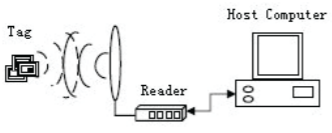
\includegraphics{schemaRFID.png}
\caption{Schema di funzionamento di un tipico sistema RFID}
\end{figure}
\section{La tecnologia RFID come valido sostituto al barcode}
Ci sono molti motivi per via dei quali la tecnologia RFID ha sostituito la più vecchia e obsoleta tecnologia barcode:
\begin{itemize}
\item Il tag non deve essere a contatto con l'interrogatore durante il trasferimento dell'informazione.
\item Il tag non deve necessariamente essere visibile per essere scritto/letto.
\item La lettura/scrittura del tag non richiede intervento umano, ne consegue che il costo per la manodopera diminuisce e l'errore umano viene minimizzato.
\item Il range di lettura/scrittura è più ampio rispetto a quello del barcode.
\item I tag possono essere riscritti/modificati e possono ospitare una maggiore quantità di dati.
\item E' più facile creare un codice univoco all'interno del tag.
\item I tag sono meno sensibili a condizioni avverse (polvere, danni fisici ecc.).
\item Più tag possono essere letti simultaneamente\cite{Kaur:RFIDTechnologyPrinciplesAdvantagesLimitationsApplications}.
\end{itemize}
\section{Applicazione in progetti IoT}
La tecnologia RFID non solo viene adoperata largamente in ambito commerciale, ma anche in altri ambiti non strettamente economici come in quello sanitario e militare. La ragione per la quale venga ancora utilizzata, nonostante abbia compiuto più di vent'anni, è data dal fatto che sappia constantemente adattarsi al cambiamento e alla costante evoluzione dell'IoT\cite{Xiaolin:RFIDTechnologyApplicationsIoT}.\\
\begin{figure}[h]
\centering
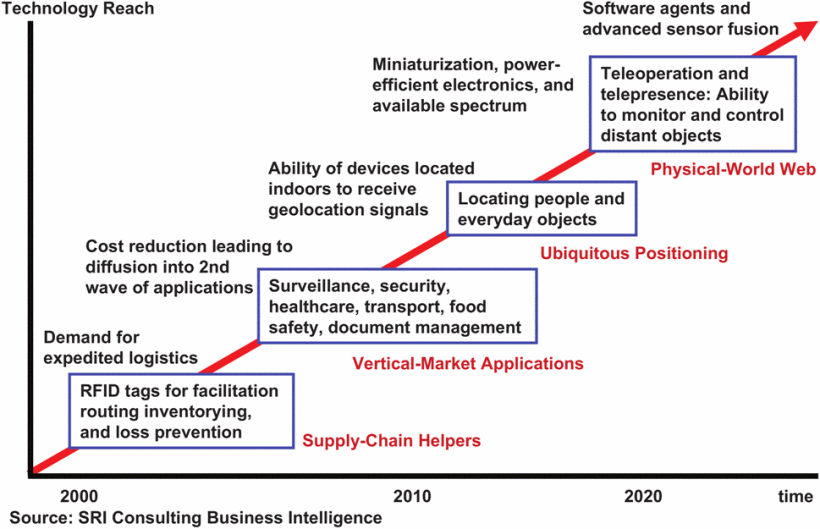
\includegraphics[scale = 0.3]{graficoRFID.png}
\caption{La tecnologia RFID si evolve con l'evolversi di IoT}
\end{figure}

\chapter{Piattaforme IoT Cloud}
\section{La nascita del Cloud Computing}
Il concetto alla base del cloud computing è stato introdotto negli anni '60 da John McCarthy. La sua opinione era che {\itshape il calcolo potrebbe un giorno essere organizzato come un servizio di pubblica utilità}.  La storia del termine cloud deriva dal mondo delle telecomunicazioni dove le suddette società hanno iniziato a offrire servizi di rete privata virtuale (VPN) con una qualità del servizio comparabile a un costo molto inferiore. Inizialmente prima della VPN, fornivano circuiti dati point-to-point dedicati, il che rappresentava uno spreco di larghezza di banda. Tuttavia, utilizzando i servizi VPN, si è potuto cambiare il traffico per bilanciare l'utilizzo della rete complessiva. Il cloud computing ora si estende ai server e all'infrastruttura di rete.
\\Molti attori del settore sono entrati nel cloud computing e lo hanno implementato. Amazon ha svolto un ruolo chiave e ha lanciato Amazon Web Service (AWS) nel 2006. Anche Google e IBM hanno avviato progetti di ricerca nel cloud computing. Eucalyptus è diventata la prima piattaforma open source per la distribuzione di cloud privati\cite{Jadeja:Cloudcomputingconceptsarchitectureandchallenges}.\\
\begin{figure}[h]
\centering
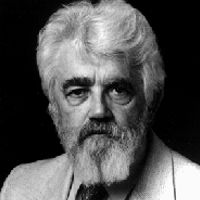
\includegraphics[scale = 0.5]{mccarthy.jpg}
\caption{John McCarthy}
\end{figure}
\newpage
\section{Definizione e funzionamento}
Una piattaforma IoT Cloud facilita l'implementazione di applicazioni software togliendone costi e complessità di acquisizione e gestione fornendo servizi avanzati mediante l'interconnessione fisica e virtuale di oggetti opportunamente configurati sfruttando un accesso di rete on-demand a un pool condiviso di risorse informatiche configurabili (ad es. reti, server, storage, applicazioni e servizi) che possono essere rapidamente fornite e rilasciate con il minimo sforzo di gestione o interazione con il fornitore di servizi\cite{Ray:AsurveyofIoTcloudplatforms}.
\section{Applicazione in progetti IoT}
L'IoT Cloud ha dato vita a una nuova serie di servizi e applicazioni intelligenti che possono avere un forte impatto sulla vita di tutti i giorni. Di seguito le principali applicazioni:
\begin{itemize}
\item Smart Home
\item Video sorveglianza
\item Assistenza sanitaria
\item Città e comunità intelligenti
\item Smart Grid\footnote{insieme di reti di informazioni e di reti di distribuzione dell’energia elettrica. È una rete detta {\itshape intelligente} in quanto ottimizza la distribuzione dell’energia elettrica}
\item Mobilità automobilistica e intelligente
\item Logistica intelligente
\item Monitoraggio ambientale\cite{Botta:IntegrationofCloudcomputingandInternetofThingsAsurvey}.
\end{itemize}
\begin{figure}[h]
\centering
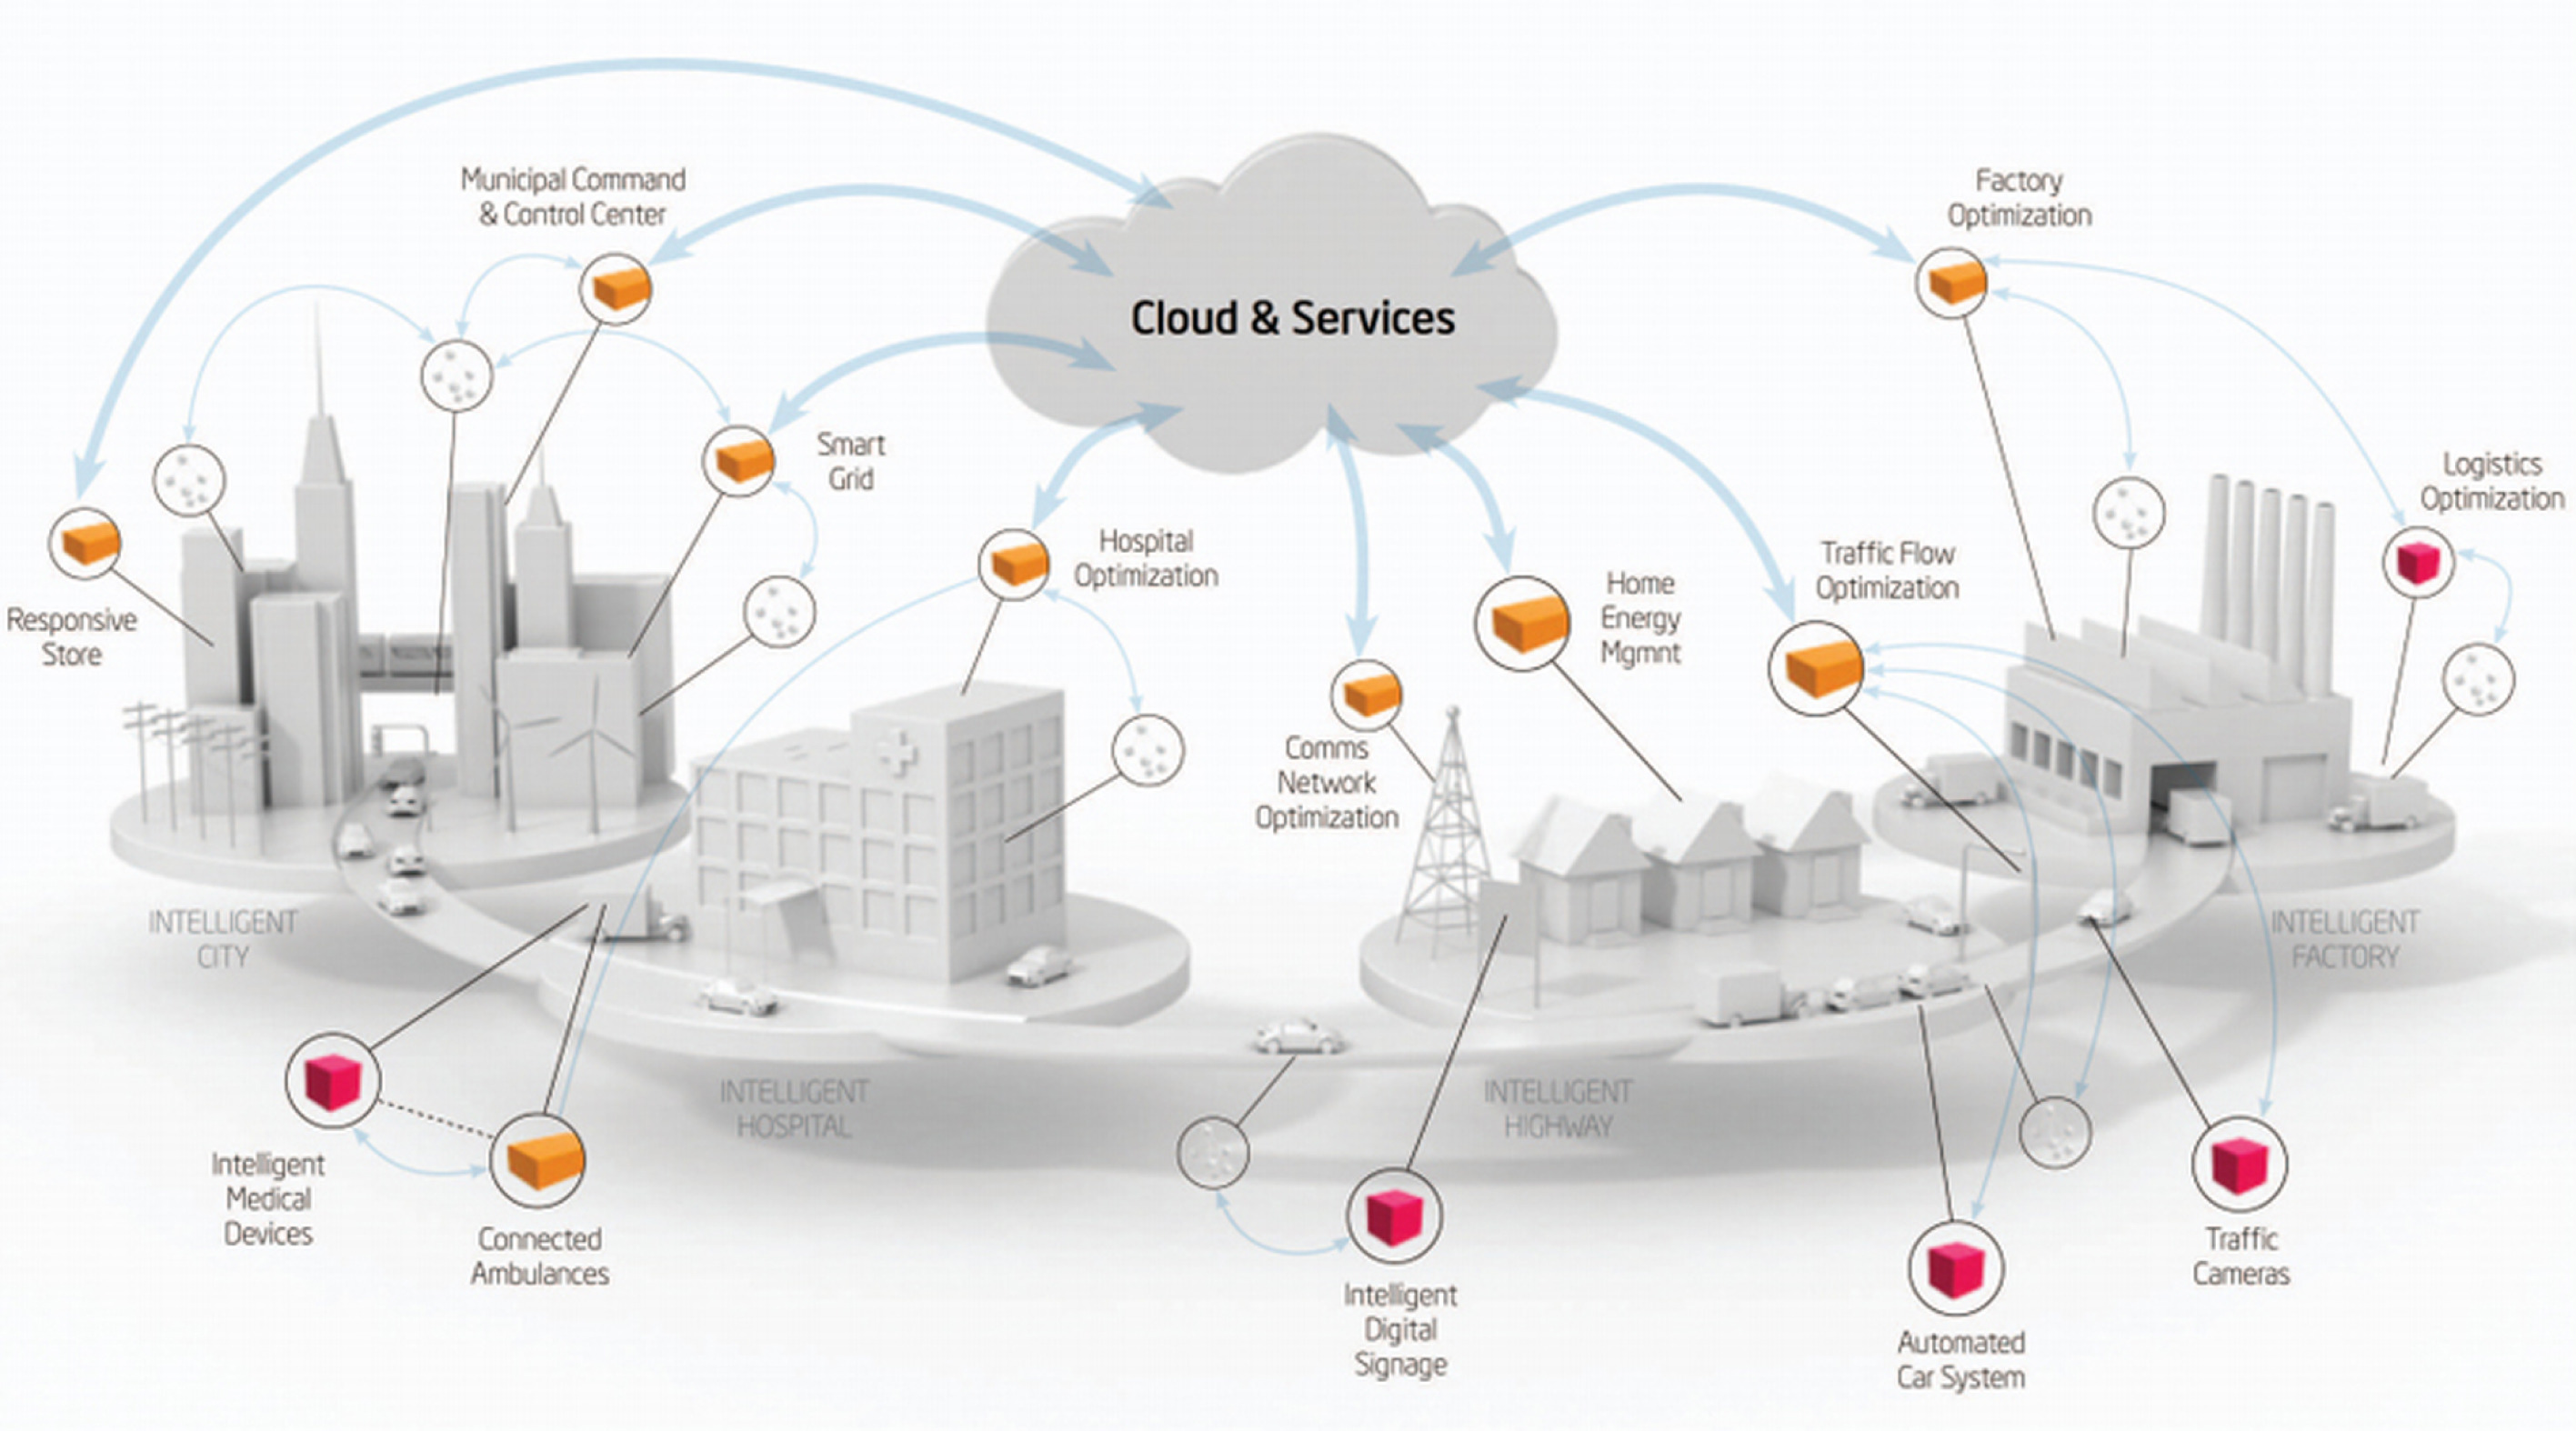
\includegraphics[scale = 0.75]{schemaCloudIoT.PNG}
\caption{Esempio di una vasta applicazione di Cloud IoT}
\end{figure}

\chapter{Arduino}
\section{La nascita di Arduino}
Il progetto Arduino è stato avviato presso l'Interaction Design Institute Ivrea (IDII) a Ivrea. Nel 2003 Hernando Barragán ha creato la piattaforma di sviluppo Wiring come progetto di tesi magistrale all'IDII, sotto la supervisione di Massimo Banzi e Casey Reas. L'obiettivo del progetto era creare strumenti semplici e a basso costo per la creazione di progetti digitali da parte di non ingegneri. La piattaforma di cablaggio consisteva in un circuito stampato\footnote{supporto utilizzato per interconnettere tra di loro i vari componenti elettronici di un circuito tramite piste conduttive incise su di un materiale non conduttivo} con un microcontrollore\footnote{dispositivo elettronico integrato utilizzato soprattutto nei sistemi embedded per applicazioni specifiche di controllo digitale} ATmega128, un IDE\footnote{ambiente di sviluppo} basato su funzioni di elaborazione e libreria per programmare facilmente il microcontrollore. Nel 2005, Massimo Banzi, con David Mellis, un altro studente IDII, e David Cuartielles, ha esteso il cablaggio aggiungendo il supporto per il microcontrollore ATmega8 più economico. Il nuovo progetto, derivato da Wiring venne chiamato Arduino\cite{Kushner:TheMakingOfArduino}.
\begin{figure}[h]
\centering
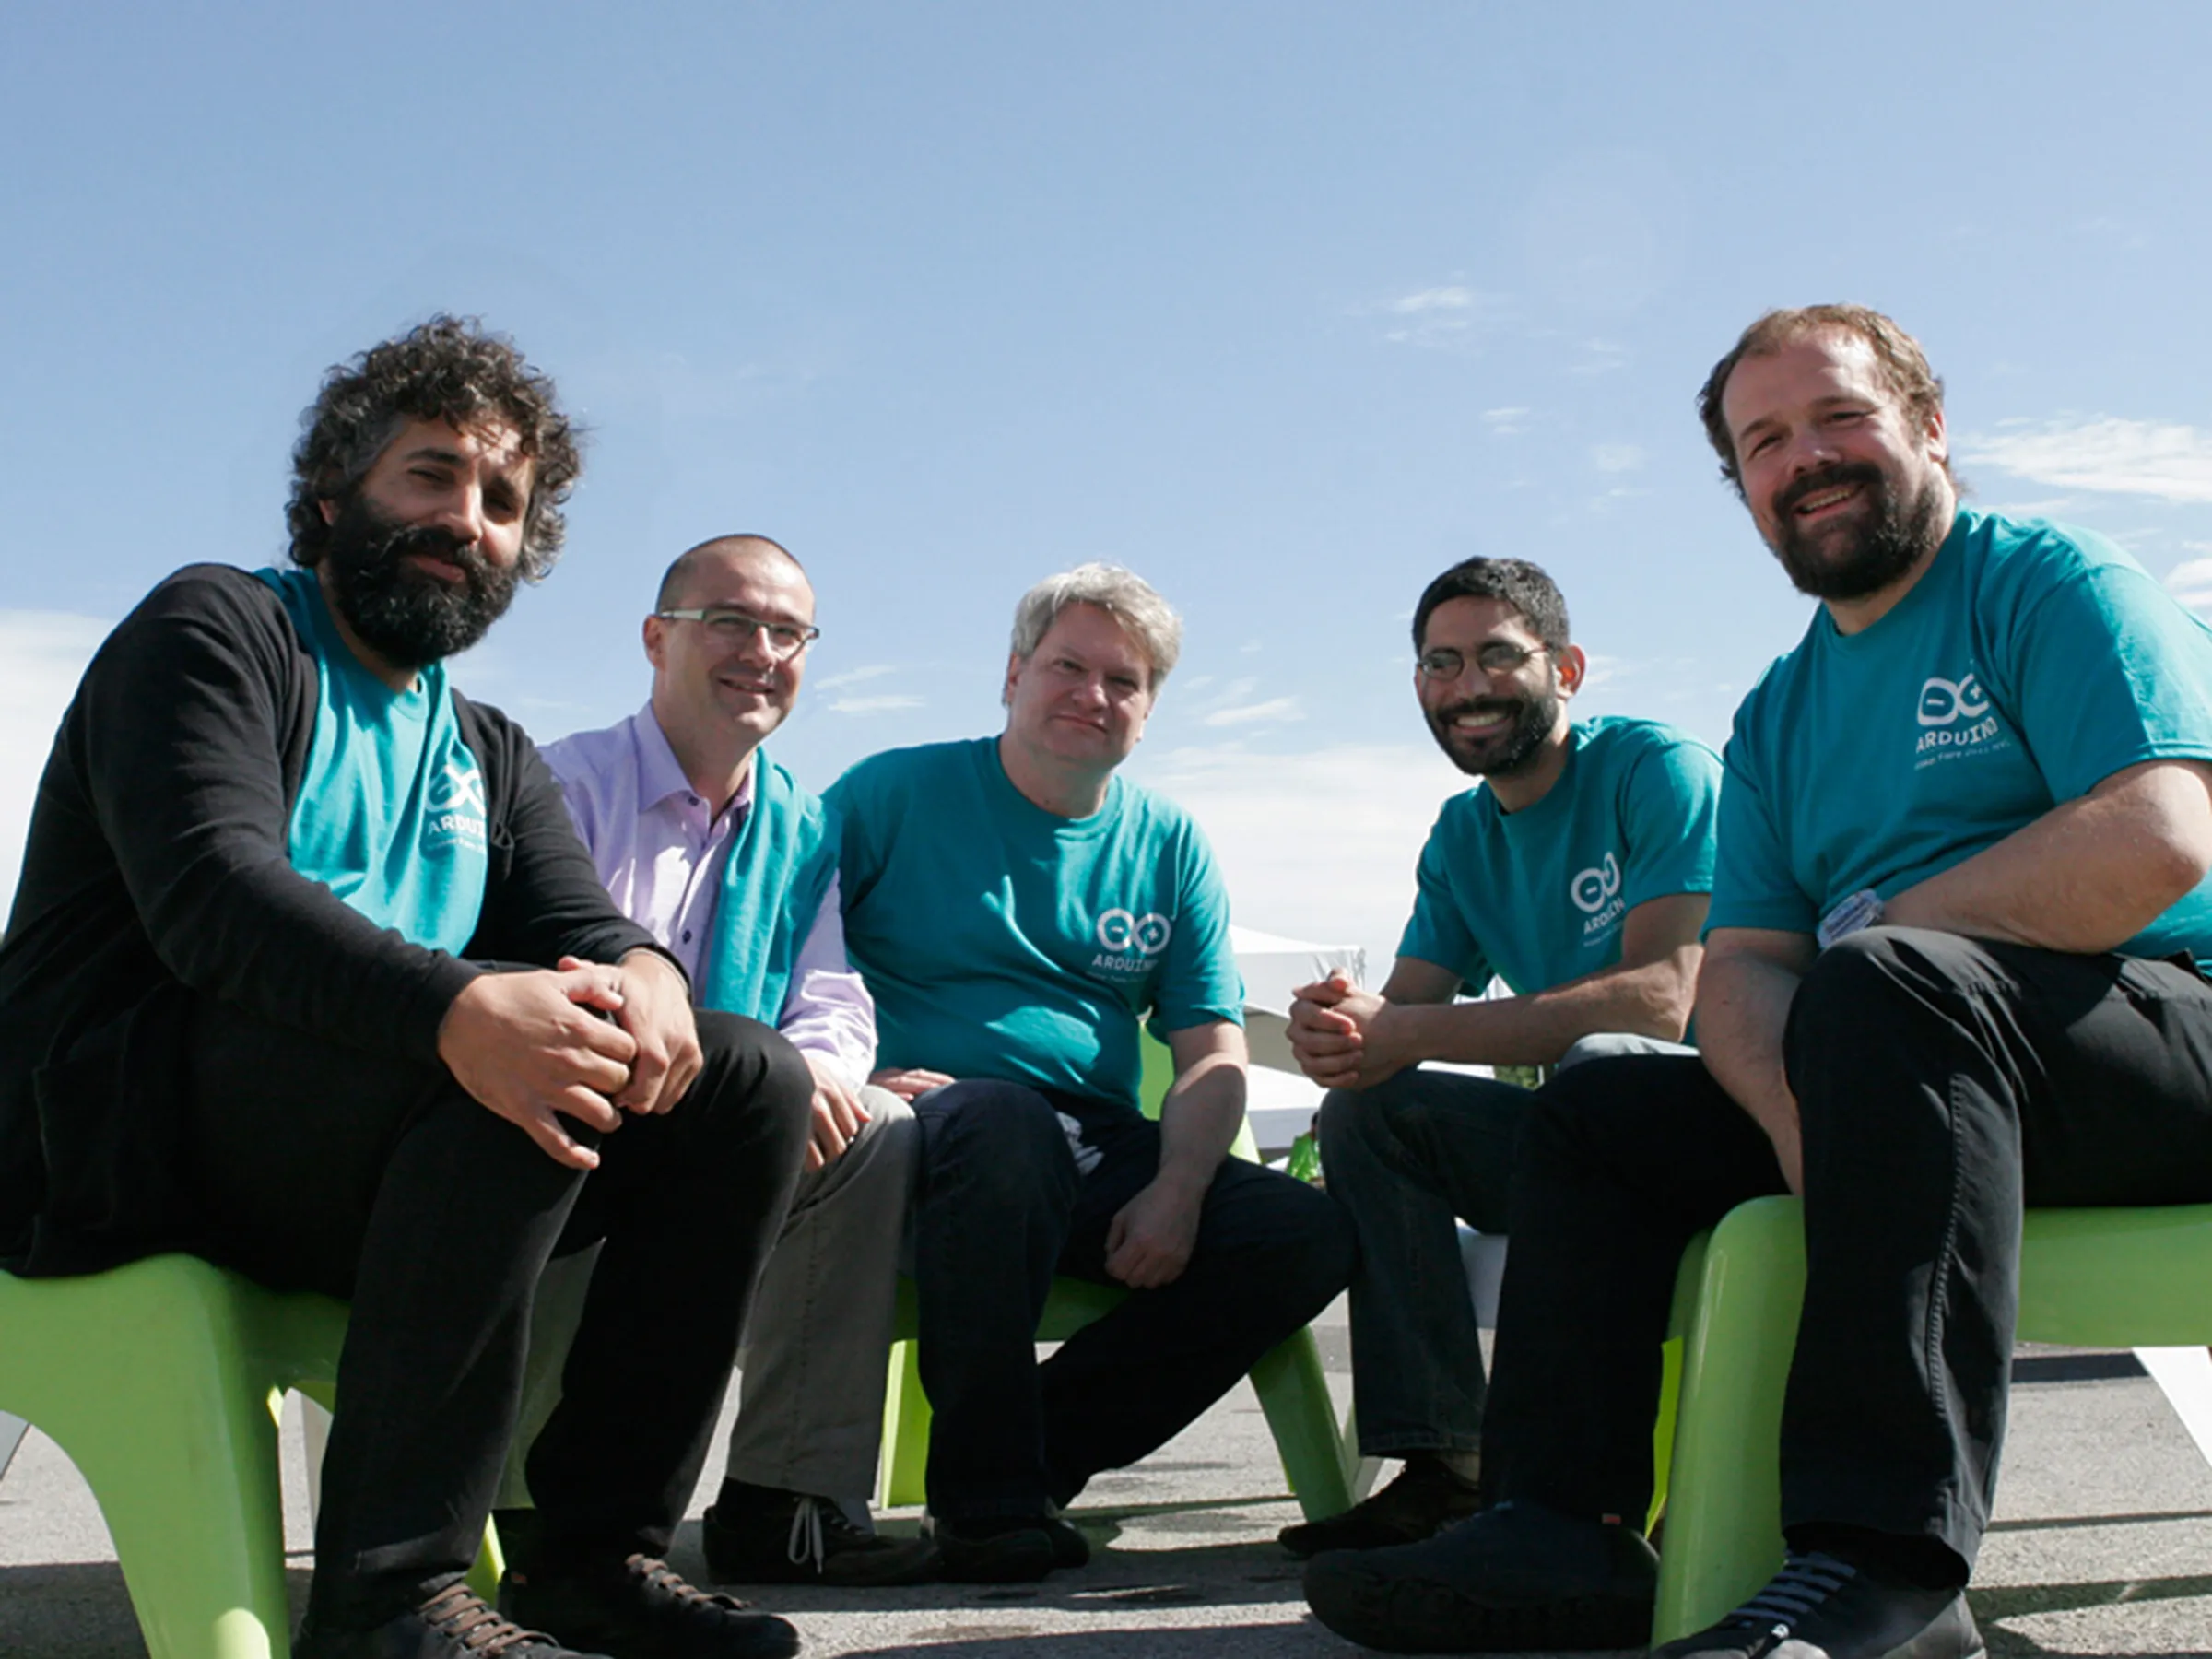
\includegraphics[scale = 0.07]{teamarduino.png}
\caption{Arduino core team (da sinistra) - David Cuartielles, Gianluca Martino, Tom Igoe, David Mellis, and Massimo Banzi}
\end{figure}
\section{Definizione e funzionamento}
Arduino è una piattaforma open-source\footnote{software rilasciato con una licenza tale da permettere agli utenti di utilizzare, studiare, modificare e distribuire il software e il suo codice sorgente a chiunque e per qualsiasi scopo} utilizzata per la costruzione e la programmazione elettronica. Può ricevere e inviare informazioni determinati dispositivi anche tramite l'ausilio di internet. A livello hardware viene utilizzata scheda elettronica mentre a livello software quest'ultima viene programmata tramite l'ausilio di un inguaggio simile al C++\footnote{estensione del linguaggio di programmazione C}.\\
Può essere programmato per eseguire numerose attività. E' necessario caricare all'interno del microcontrollore Arduino i comandi specificati dall'utente per eseguire il task specifico. Un arduino può aiutare a leggere le informazioni dai dispositivi di input come ad esempio sensori e antenne e può anche inviare informazioni a dispositivi di output come LED, altoparlanti, schermi LCD e motori\cite{Badamasi:TheworkingprincipleofanArduino}.\\
Tutte le schede Arduino possiedono degli ingressi Input/Output chiamati {\itshape pin} che vengono utilizzati per interfacciarsi con i vari componenti. I pin vengono chiamati digitali se ragionano in termini di LOW/HIGH (0/1) o analogici se ragionano in un range di valori compreso fra 0 e 1023. La scheda Arduino più utilizzata al mondo {\itshape Arduino Uno} possiede 14 pin digitali e 6 pin analogici\cite{Caccavale:NozionisuInputOutputArduino}. \\\\
\begin{figure}[h]
\centering
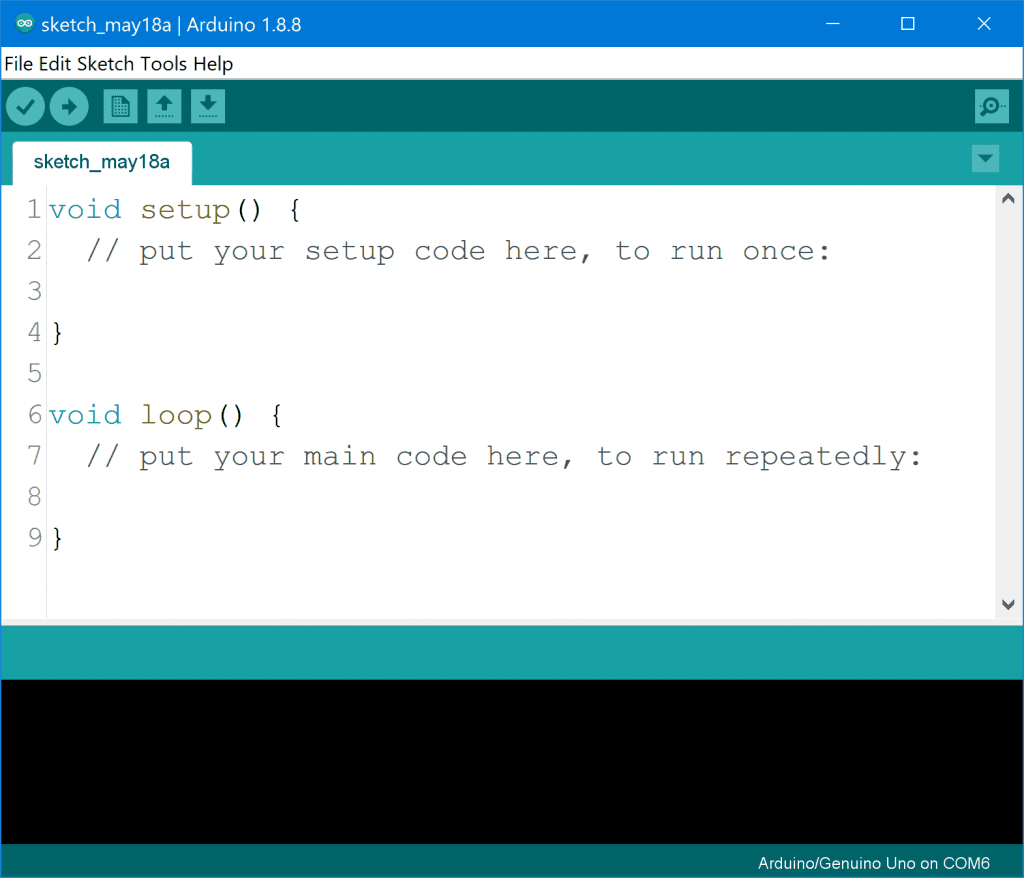
\includegraphics[scale = 0.2]{ide.png}
\caption{L'ambiente di sviluppo Arduino}
\end{figure}
\begin{figure}[h]
\centering
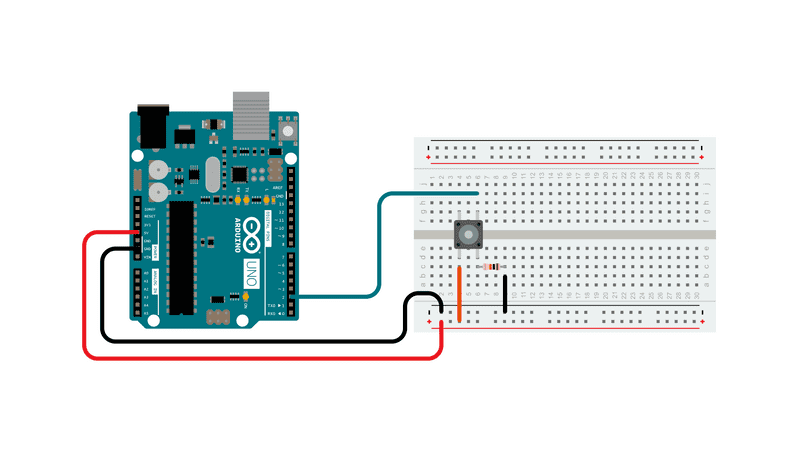
\includegraphics[scale = 0.3]{circuit.png}
\caption{Schema di un circuito rappresentante una scheda a cui è stato collegato un bottone}
\end{figure}
\begin{figure}[h]
\centering
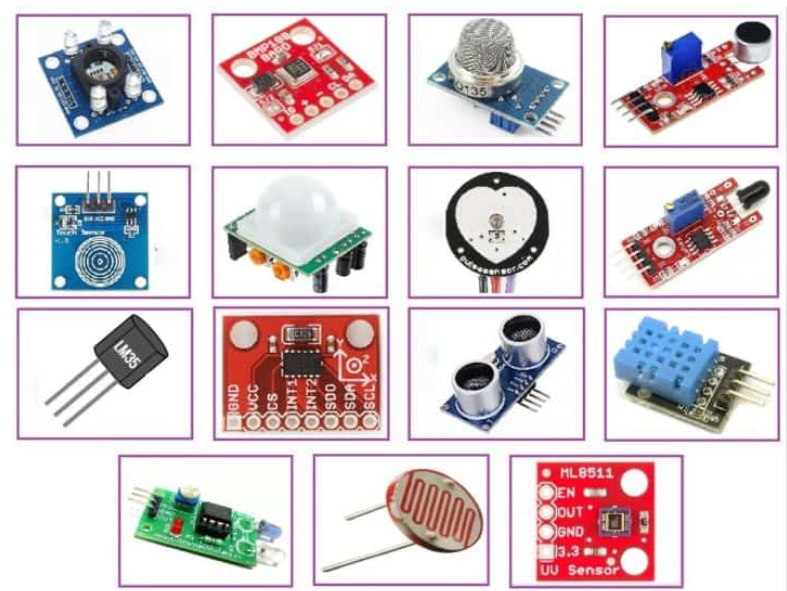
\includegraphics[scale = 0.3]{sensors.png}
\caption{15 sensori importanti (da in alto a sinistra) - Sensore dei colori, sensore della pressione barometrica, sensore del battito cardiaco, rilevatore di gas/alcol/fumo, sensore della temperatura, sensore del suono, rilevatore di fumo/fuoco, sensore di tocco, sensore di infrarossi passivo, accelerometro, sensore ultrasonico, sensore d'umidità, sensore di infrarossi, sensore di luce, sensore di raggi UV}
\end{figure}

\chapter{Progetto di Smart Parking}
\section{Introduzione}
Ora che sono state poste le basi su IoT e suddette possibili implementazioni è possibile proseguire con la spiegazione del progetto, argomento principale della tesi.\\
Il progetto di Smart Parking in oggetto si propone di fornire una soluzione efficiente alla gestione di un parcheggio al fine di velocizzare il processo di entrata e di uscita eliminando inutili code al casello sfruttando pagamenti elettronici e sensori in grado di riconoscere il veicolo in entrata e in uscita. ll sistema inoltre prevede all'utente una visione dello storico dei pagamenti effettuati in precedenza.

\begin{figure}[h]
\centering
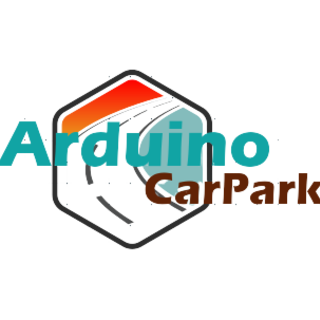
\includegraphics[scale = 0.7]{logo.png}
\caption{logo del progetto}
\end{figure}

\newpage
\section{Struttura del progetto}
\begin{figure}[h]
\centering
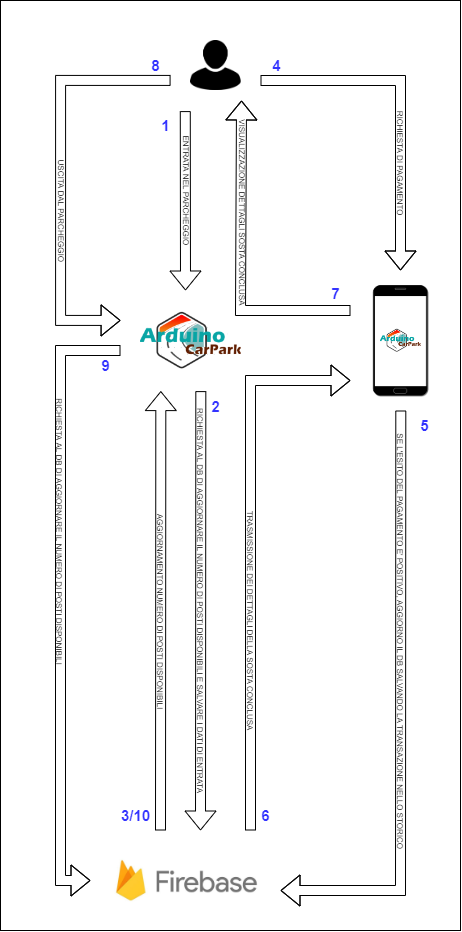
\includegraphics[scale = 0.498]{struttura.png}
\end{figure}
\newpage
\section*{Il prototipo}
\begin{figure}[h]
\centering
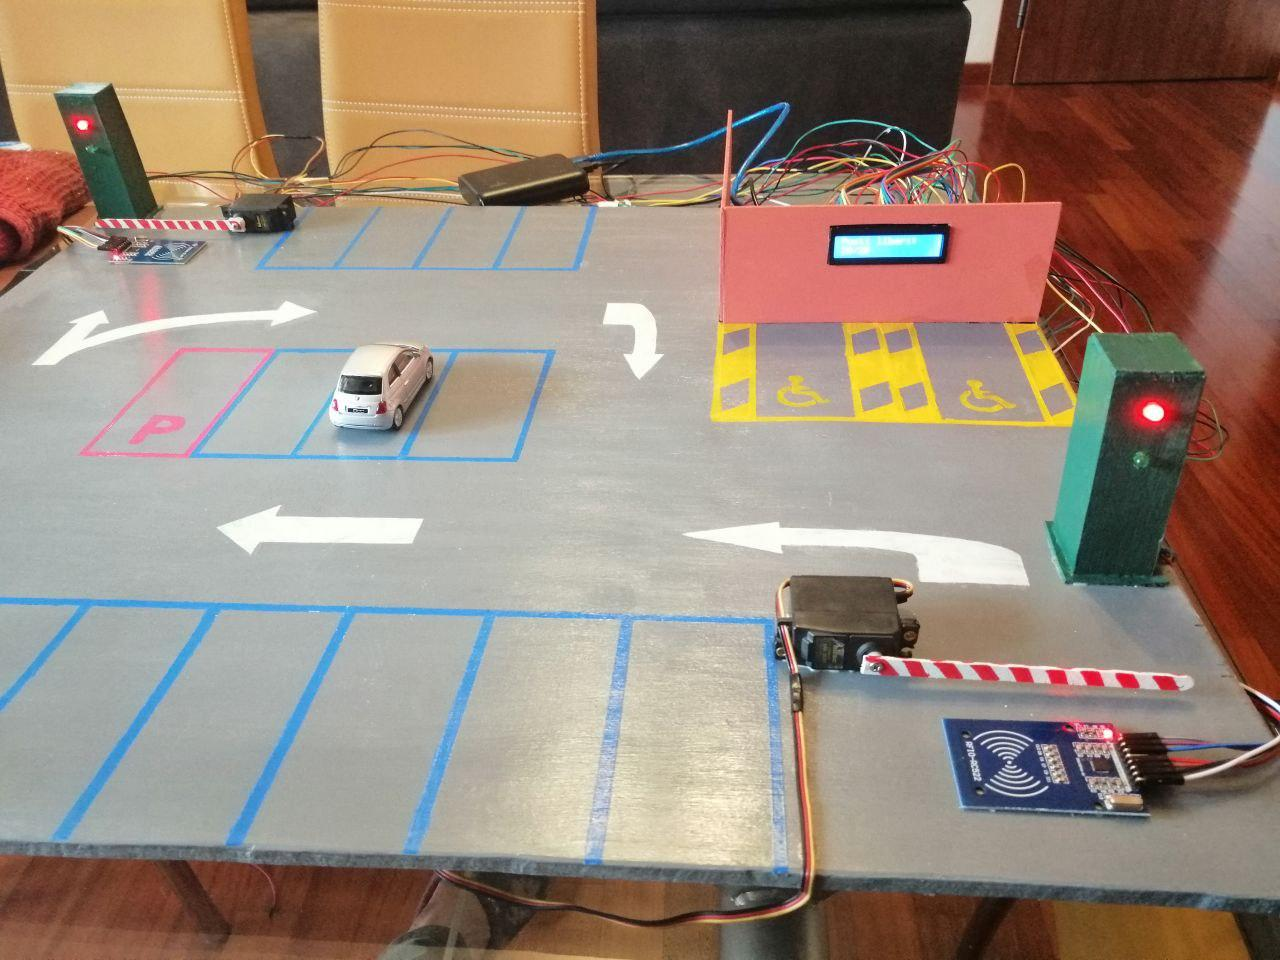
\includegraphics[scale = 0.25]{progetto.jpg}
\caption{Vista frontale del prototipo}
\end{figure}
La necessità di dover implementare molti componenti importanti in termini di spazio fra cui sensori rfid, motori e display LCD è stata decisiva per la scelta della scheda da utilizzare. Per questo scopo infatti si vedeva necessario disporre di una scheda più capiente e performante rispetto alla classica {\itshape Arduino Uno} e la scelta è ricaduta sulla scheda {\itshape Arduino Mega 2560}.\\
\begin{table}[htb]
\caption{Specifiche tecniche}
\vspace{4mm}
\centering
\hspace*{-0.9in}
\begin{tabular}{l c}
\toprule
\textbf{Specifica} & \textbf{Valore} \\
\midrule
\textbf{Microcontrollore} & ATMega2560 \\
\textbf{Tensione di esercizio} & 5V \\
\textbf{Tensione di input raccomandata} & 7-12V \\
\textbf{Pin digitali} & 54 \\
\textbf{Pin analogici} & 16 \\
\textbf{Memoria Flash*} & 256 KB \\
\textbf{SRAM**} & 8 KB \\
\bottomrule
{\small *memoria utilizzata dalla scheda per immagazzinare il codice dello sketch una volta compilato.}\\
{\small **tipo di RAM che contiene i dati in una forma statica, cioè finché la memoria è alimentata.}
\end{tabular}
\end{table}
\newpage
\begin{figure}[h]
\centering
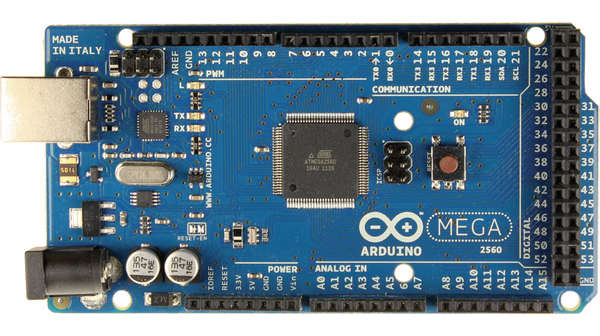
\includegraphics[scale = 0.498]{scheda.jpg}
\caption{scheda Arduino Mega 2560}
\end{figure}
Il lettore utilizzato per identificare ogni singolo veicolo entrante o uscente legge tag con identificazione a radio frequenza. Il suo nome tecnico è {\itshape lettore RFID RC522}.
\begin{figure}[h]
\centering
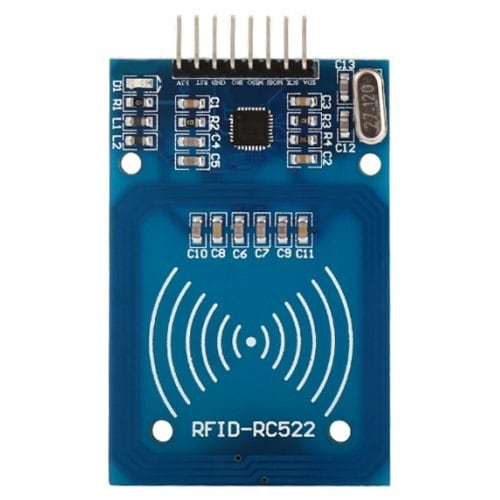
\includegraphics[scale = 0.3]{rfid.jpg}
\caption{lettore RFID RC522}
\end{figure}
\newpage
Attraverso la scheda {\itshape NodeMCU 1.0} , è possibile interfacciare Arduino all’IoT. Più in particolare, la scheda rende possibile la comunicazione fra Arduino e il Database in cloud dove vengono immagazzinati i dati delle soste correnti e concluse.
\begin{figure}[h]
\centering
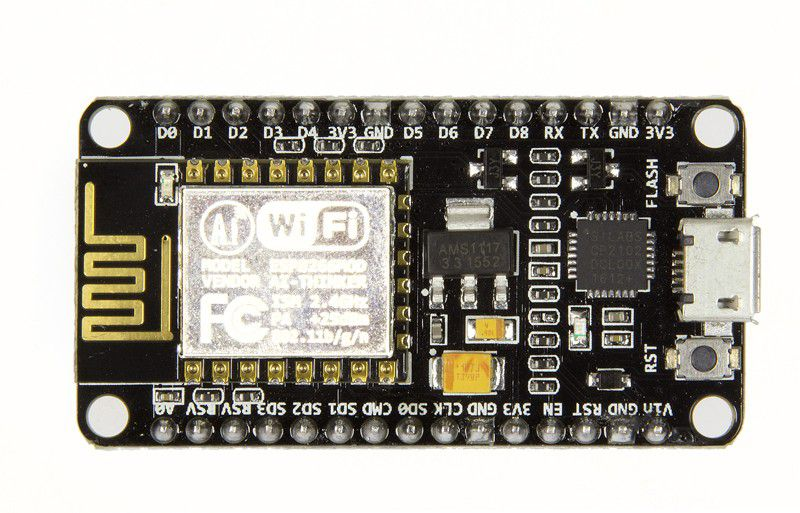
\includegraphics[scale = 0.3]{nodemcu.jpg}
\caption{NodeMCU 1.0}
\end{figure}

Ad informare gli utenti dei posti disponibili nel parcheggio, è stato installato un display LCD 16x2 che raffigura i posti disponibili.\\
Dei servo motori sono stati utilizzati per costruire le barre automatiche di ingresso.\\
In ultima battuta sono stati utilizzati dei led per simulare dei semafori di uscita/entrata.

\begin{figure}[!htb]
\minipage{0.32\textwidth}
  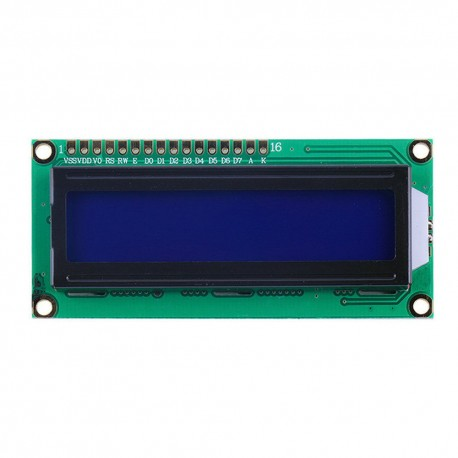
\includegraphics[width=\linewidth]{display.jpg}
  \caption{display LCD 16x2}
\endminipage\hfill
\minipage{0.32\textwidth}
  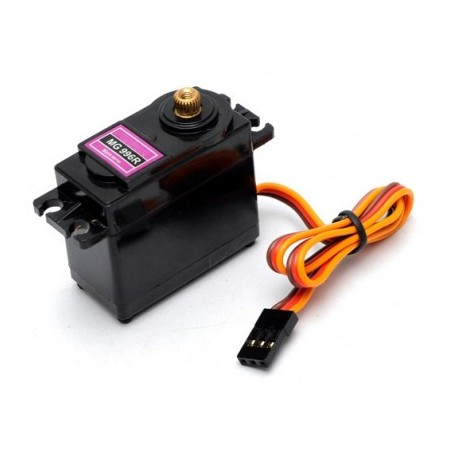
\includegraphics[width=\linewidth]{servo.jpg}
  \caption{servo motore}
\endminipage\hfill
\minipage{0.32\textwidth}%
  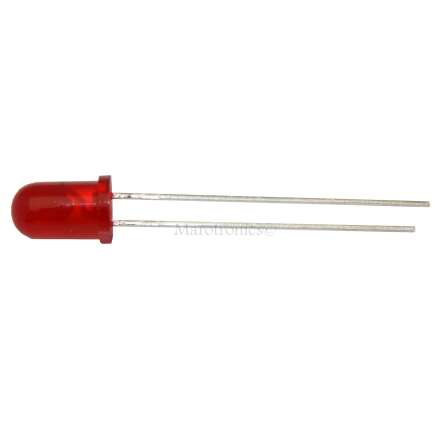
\includegraphics[width=\linewidth]{led.jpg}
  \caption{led}
\endminipage
\end{figure}

\newpage
\section*{La base dati}
{\itshape Firebase} è una piattaforma open source sviluppata da Google per lo sviluppo di applicazioni mobili e web.\\
Essa fornisce una suite di strumenti per scrivere, analizzare e mantenere applicazioni cross-platform\footnote{applicazioni programmate per girare su più piattaforme}. {\itshape Firebase} infatti offre funzionalità come analisi e storage dati all'interno di database aventi strutture NoSql\footnote{database che memorizzano i dati in un formato diverso dalle tabelle relazionali}.
\begin{figure}[h]
\centering
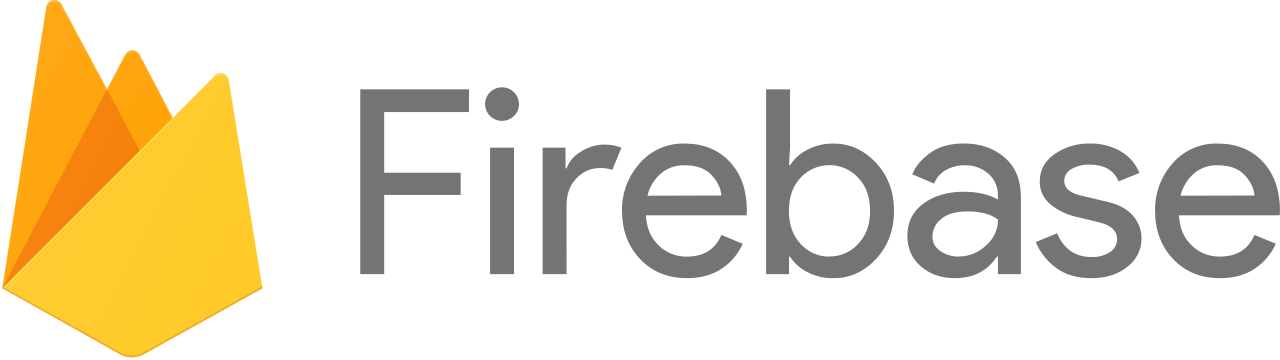
\includegraphics[scale = 0.1]{firebase.png}
\caption{logo di {\itshape Firebase}}
\end{figure}

All'interno del database sono salvati i dettagli della sosta per ciascun utente specificando l'id dell'utente, il flag di pagamento (true se pagato, false se da pagare), il timestamp di arrivo e di uscita e infine il prezzo calcolato in base al tempo di sosta.
\begin{figure}[h]
\centering
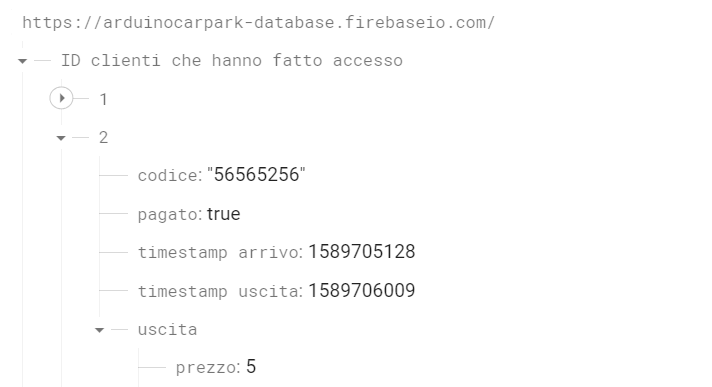
\includegraphics[scale = 0.7]{database_1.png}
\caption{dettagli della sosta}
\end{figure}

Inoltre sono salvate le informazioni generali sulla disponibilità dei posti nel parcheggio.
\begin{figure}[h]
\centering
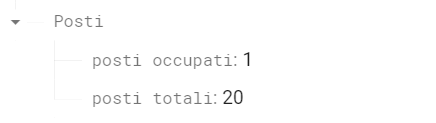
\includegraphics[scale = 0.7]{database_2.png}
\caption{indicazione dei posti occupati e dei posti totali}
\end{figure}
\newpage
\section*{L'applicazione}
L'applicazione scritta interamente in Java permette all'utente di pagare la sosta in modo comodo e veloce via smartphone tramite Paypal e visualizzare lo storico delle precedenti soste presso il parcheggio.\\
All'apertura dell'applicazione vi è la schermata di login a cui ciascun utente potrà accedere con le proprie credenziali. Una volta effettuato l'accesso sarà accessibile la visione dello storico soste riguardante il singolo utente e se il sistema rileverà una sosta in corso renderà visibile la procedura per iniziare il processo di pagamento della sosta. Si aprirà dunque la schermata di pagamento tramite Paypal che gestirà la riscossione del denaro in base al prezzo calcolato dal sistema in base al tempo della sosta.

\begin{figure}[h]
\centering
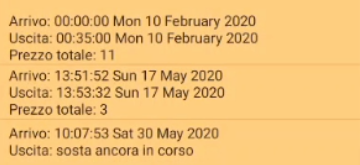
\includegraphics[scale = 1]{storico.png}
\caption{storico delle soste}
\end{figure}

\begin{figure}[!htb]
\minipage{0.32\textwidth}
  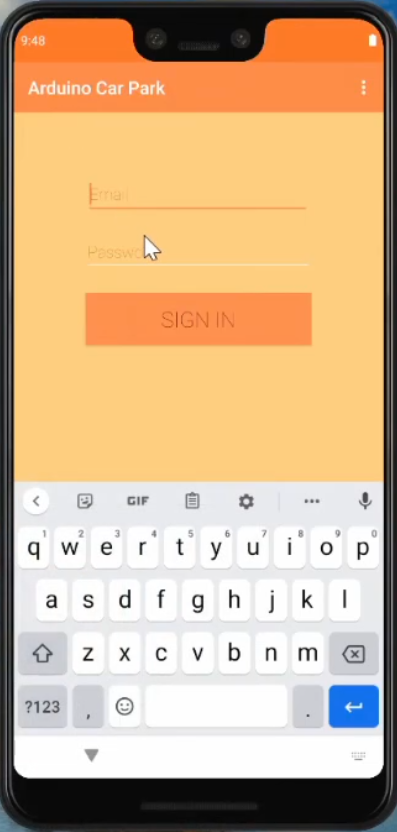
\includegraphics[width=\linewidth]{app_1.png}
  \caption{schermata di login}
\endminipage\hfill
\minipage{0.32\textwidth}
  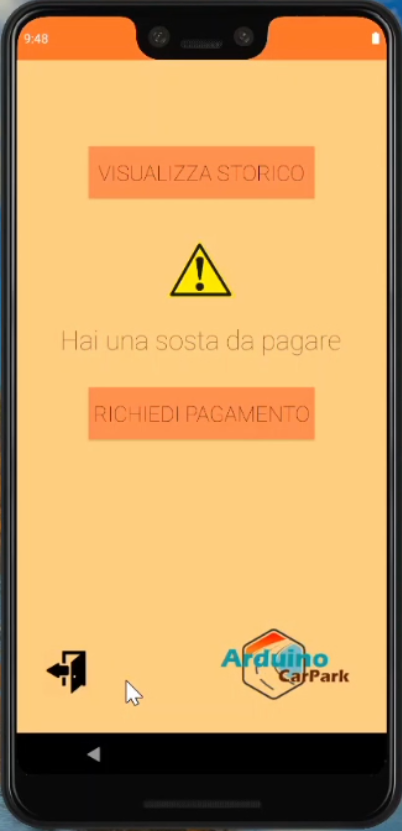
\includegraphics[width=\linewidth]{app_2.png}
  \caption{sosta da pagare}
\endminipage\hfill
\minipage{0.32\textwidth}%
  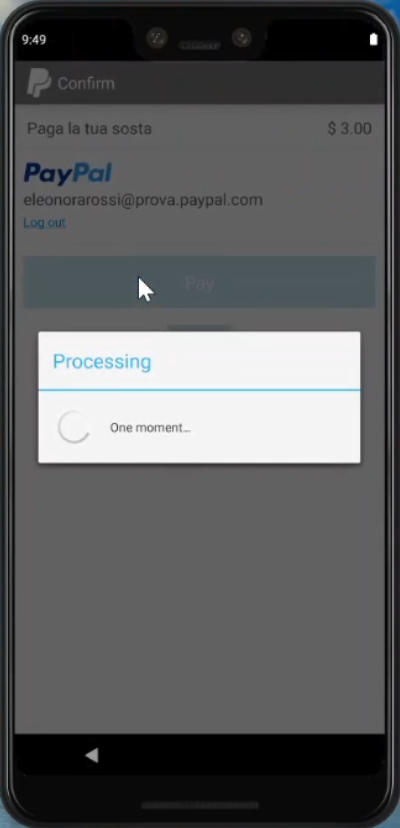
\includegraphics[width=\linewidth]{app_3.png}
  \caption{pagamento in corso}
\endminipage
\end{figure}

\newpage
\section{Flowchart di funzionamento}
Di seguito, uno schematico flowchart che spiega nel dettaglio le operazioni svolte dal sistema
\begin{figure}[h]
\centering
\hspace*{-1.5in}
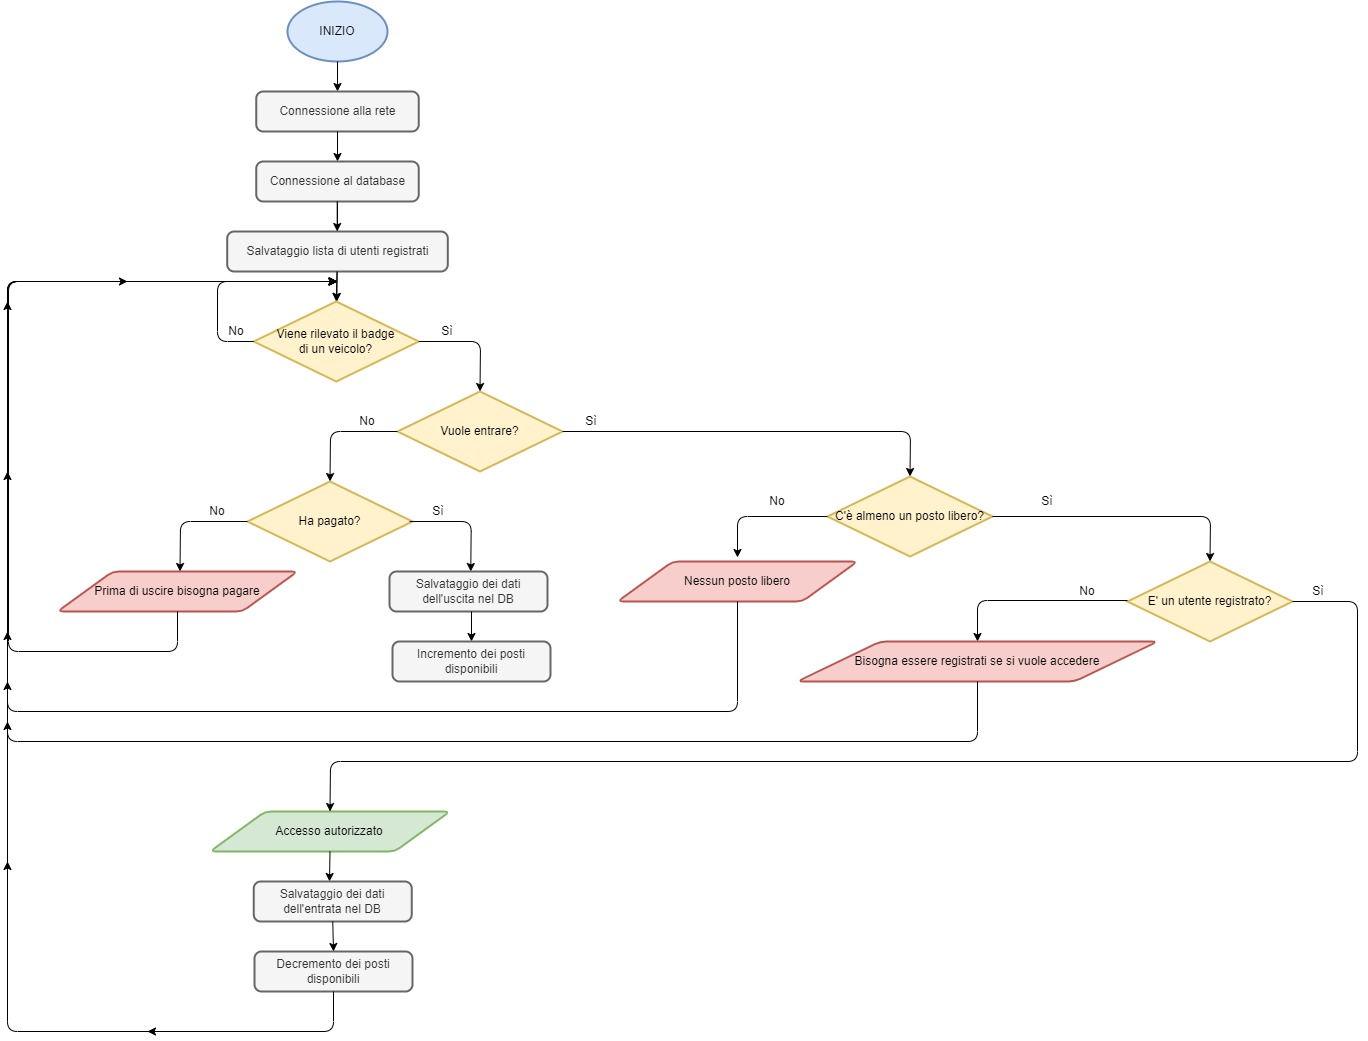
\includegraphics[scale = 0.41]{flowchart.jpg}
\end{figure}

\newpage
\section{Link del progetto}
\begin{itemize}
\item Video YouTube che spiega il funzionamento del progetto\\
\textbf{ArduinoCarPark: an Arduino/Android project of a car park}\\
\url{ https://www.youtube.com/watch?v=rVw_7KriAOk&ab_channel=AuroraBussola}
\item Repository GitHub del progetto\\
\textbf{ArduinoCarPark}\\
\url{ https://github.com/exogenesis18/ArduinoCarPark}
\end{itemize}

% Bibliografia
\begin{thebibliography}{99}
\bibitem{Ansari:BasedHealthcareApplications}
Seema Ansari, Tahniyat Aslam, Javier Poncela, Pablo Otero, Adeel Ansari,
\emph{introduzione di Internet of Things-Based Healthcare Applications},
\url{https://www.igi-global.com/chapter/internet-of-things-based-healthcare-applications/243907}.
\bibitem{Ashton: ThatInternetofThings'Thing}
Kevin Ashton,
\emph{That 'Internet of Things' Thing},
\url{http://www.itrco.jp/libraries/RFIDjournal-That%20Internet%20of%20Things%20Thing.pdf}.
\bibitem{Feng:InternationJournalOfCommunicationSystems}
Feng Xia, Laurence T. Yang, Lizhe Wang, Alexey Vinel,
\emph{Internation Journal Of Communication Systems.}
\bibitem{Suresh:StateArtReviewIoTHistoryTechnologyFieldsDeployment}
P. Suresh, J. Vijay Daniel, V. Parthasarathy, R. H. Aswathy,
\emph{A state of the art review on the Internet of Things (IoT) history, technology and fields of deployment}
\url{https://ieeexplore.ieee.org/abstract/document/7043637}.
\bibitem{Sun:ApplicationRFIDTechnologyLogisticsInternetofThings}
Chunling Sun,
\emph{Application of RFID Technology for Logistics on Internet of Things}
\url{https://www.sciencedirect.com/science/article/pii/S2212671612000200}.
\bibitem{Kaur:RFIDTechnologyPrinciplesAdvantagesLimitationsApplications}
Mandeep Kaur, Manjeet Sandhu, Neeraj Mohan, Parvinder S. Sandhu,
\emph{RFID Technology Principles, Advantages, Limitations And Its Applications}
\url{http://ijcee.org/papers/306-E794.pdf}
\bibitem{Xiaolin:RFIDTechnologyApplicationsIoT}
Xiaolin Jia, Quanyuan Feng, Taihua Fan, Quanshui Lei,
\emph{RFID technology and its applications in Internet of Things (IoT)}
\url{https://ieeexplore.ieee.org/abstract/document/6201508}
\bibitem{Jadeja:Cloudcomputingconceptsarchitectureandchallenges}
Yashpalsinh Jadeja, Kirit Modi,
\emph{Cloud computing - concepts, architecture and challenges}
\url{https://ieeexplore.ieee.org/abstract/document/6203873}
\newpage
\bibitem{Ray:AsurveyofIoTcloudplatforms}
Partha Pratim Ray,
\emph{A survey of IoT cloud platforms}
\url{https://www.sciencedirect.com/science/article/pii/S2314728816300149}
\bibitem{Botta:IntegrationofCloudcomputingandInternetofThingsAsurvey}
Alessio Botta, Walter de Donato, Valerio Persico, Antonio Pescapé,
\emph{Integration of Cloud computing and Internet of Things: A survey}
\url{https://www.sciencedirect.com/science/article/pii/S0167739X15003015}
\bibitem{Kushner:TheMakingOfArduino}
David Kushner,
\emph{The Making Of Arduino}
\url{https://spectrum.ieee.org/the-making-of-arduino}
\bibitem{Badamasi:TheworkingprincipleofanArduino}
Yusuf Abdullahi Badamasi,
\emph{The working principle of an Arduino}
\url{https://ieeexplore.ieee.org/abstract/document/6997578}
\bibitem{Caccavale:NozionisuInputOutputArduino}
Giuseppe Caccavale,
\emph{Nozioni su Input/Output – Arduino}
\url{https://www.giuseppecaccavale.it/corso-arduino/nozioni-su-input-output/}
\end{thebibliography}

\end{document}

